\section{Application}

% Introduction {{{
Our goal was to make use of a lot of computing power in
order to train our agent to master an OpenAI Gym
Environment (cmp. \ref{s_openai_gym}). In this chapter we
will document how we tried to achieve this goal with our
distributed application.
\index{Application}

% }}}

% The agent {{{
\subsection{The agent}
\label{s_agent}

Before going into detail on the application's architecture,
here is a brief summary on what our agent actually is.

We programmed our agent as a neural network with the Keras
library, which has an API for high level, high abstraction
neural networks.

Keras uses Tensorflow as its backend for computations and
basically only provides a nicer abstraction of Tensorflow.

% example {{{
\begin{mdframed}[style=codebox]
\begin{lstlisting}[language=Python]
# a small example program using Keras
#
# API documentation at: https://keras.io/

# Sequential is the keras object representing a neural net-
# work
from keras.models import Sequential
# a neural net is comprised of layers connected with each
# other. The Dense object represents a layer
from keras.layers import Dense

# the neural net. This specific neural net has four layers
# (the input (size of 12), two hidden (both 64 artificial
# neurons) and the output layer (size of 4)). The input
# layer does not have to be specified since the input_dim
# parameter of the first layer automatically generates the
# input layer.
model = Sequential([
  Dense(64, activation='relu', input_dim=12 ),
  Dense(64, activation='relu'               ),
  Dense(4,  activation='softmax'            ),
])

# define how the model should learn and some other meta
# information for the training process (learning algorithm,
# optimizer, etc)
model.compile(
        optimizer = 'adam',
        loss      = 'categorical_crossentropy',
        metrics   = ['accuracy']
)

# generate a dummy data set with corresponding labels with
# 1000 entries for training
import numpy as np

data   = np.random.random((1000,12))
# generating the labels (either a 0 or a 1)
labels = np.random.randint(2, size=(1000, 1))

# training the model, iterating 10 times
model.train(data, labels, epochs=10)

# using the neural net to predict the label of a random
# data point
test   = np.random.random((1,12))

model.predict(test)
\end{lstlisting}
\end{mdframed}
\begin{figure}[H]
\caption{A small example program using Keras}
\end{figure}
% }}}

Our agent has the observation provided by the Gym
environment (cmp. \ref{s_openai_gym}) as its input
parameters and as output parameters the actions (the size
of the output layer equals the action space $a$
($|[0..a[| = a$) of the Gym environment.

% }}}


\newpage

\subsection{Architecture}

This chapter will describe in detail how our application
is build, how it works and what we use to achieve
concurrency.

On a higher level our application is devided into two
distinct parts, the Executor ($E$) and the Worker ($W$).

$E$ is the part of our application that is doing the
training and testing of our agent, while  $W$ generates
training data which is sent via the RabbitMQ to $E$ so $E$
can train the agent with this data. After training $E$
sends the agent to $W$ so $W$ can generate new training
data with the updated agent.

This iteration is continued until the agent is able to
solve the Gym environment (cmp. \ref{s_openai_gym}).

% Network {{{
\subsubsection{Network}

Instances of both, $E_i$ and $W_j$ communicate over a
message broker, in this case RabbitMQ (cmp.
\ref{s_message_broker}, \ref{s_rabbitmq}).

\begin{figure}[H]
\begin{center}
\begin{tikzpicture}

  \node[inner sep=15pt]
    at (0,0) (rmq) {};

  \node [label=$W_2$, inner ysep=50pt, above=4cm of rmq]
    (w_two) {};
  \draw[-{Stealth[color=white,length=10mm]}]
    (w_two.center) -- (rmq);
  \PCIcon{w_two}{scale=.25}

  \node [label=$W_1$, inner ysep=50pt, left =2cm of w_two]
    (w_one)   {};
  \draw[-{Stealth[color=white,length=10mm]}]
    (w_one.center) -- (rmq);
  \PCIcon{w_one}{scale=.25}

  \node [label=$W_0$, inner ysep=50pt, left =2cm of w_one]
    (w_zero)   {};
  \draw[-{Stealth[color=white,length=10mm]}]
    (w_zero.center) -- (rmq);
  \PCIcon{w_zero}{scale=.25}

  \node [right=2cm of w_two] (w_dots) {\dots};

  \node [label=$W_n$, inner ysep=50pt, right=2cm of w_dots]
    (w_n) {};
  \draw[-{Stealth[color=white,length=10mm]}]
    (w_n.center) -- (rmq);
  \PCIcon{w_n}{scale=.25}


  \node [label={below:$E_2$}, inner ysep=40pt,
    below=4cm of rmq]
    (e_two) {}
    edge[-{Stealth[color=white,length=10mm]}] (rmq);
  \PCIcon{e_two}{scale=.25}

  \node [label={below:$E_1$}, inner ysep=40pt,
    left =2cm of e_two]
    (e_one)   {}
    edge[-{Stealth[color=white,length=10mm]}] (rmq);
  \PCIcon{e_one}{scale=.25}

  \node [label={below:$E_0$}, inner ysep=40pt,
    left =2cm of e_one]
    (e_zero)   {}
    edge[-{Stealth[color=white,length=10mm]}] (rmq);
  \PCIcon{e_zero}{scale=.25}

  \node [right=2cm of e_two] (e_dots) {\dots};

  \node [label={below:$E_m$}, inner ysep=40pt,
    right=2cm of e_dots]
    (e_n) {}
    edge[-{Stealth[color=white,length=12mm]}] (rmq);
  \PCIcon{e_n}{scale=.25}


  \node[label={below:RabbitMQ},inner ysep=15pt]
    at (0,0) {};
  \RabbitMQ{rmq}{scale=.25}

\end{tikzpicture}
\end{center}
\caption{Architecture of our Application on the network
  level}
\end{figure}

% }}}


\subsubsection{Executor}
\label{s_executor}
\index{Application!Executor}

The Executor $E$ is the part of the application that is
doing the training and testing of our agent. Training and
testing is done incrementally in a loop, the "TTSL"
(Training-Testing-Sending-Loop). An Executor instance
$E_i$ gets provided with its training data from the Worker
instances $W_j$ it is connected to (via the RabbitMQ).

If the testing part of the "TTSL" failed $E_i$ sends the
newly trained agent to every $W_j$ (the sending part of the
"TTSL"). Else if the testing was successful and the agent
mastered the environment (cmp \ref{s_openai_gym}) it sends
a message that testing was successful which kills every
$W_j$.

The Executor is composed of three processes, the main
process, the meta process and the TTSL process.

\begin{itemize}[label={}]

  \item \textbf{main process:}

        The main process first initializes global shared
        variables and constants it shares with the other
        two processes. Then it starts the meta process and
        the TTSL process.

        After that the main process becomes a listener
        which listens for incoming data from the Worker
        instances connected to the RabbitMQ. If new data
        comes in it is saved in a shared variable so the
        TTSL process can access it.
        \index{Application!Executor!main process}

  \item \textbf{TTSL process:}

        The process executing the TTSL.
        \index{Application!Executor!TTSL process}

  \item \textbf{meta process:}

        This process is a listener (like main becomes after
        initializing the shared memory and starting this
        and the TTSL process) which listens to a queue
        of the RabbitMQ so this Executor can communicate
        with the Workers it is connected to.
        \index{Application!Executor!meta process}

\end{itemize}

\begin{figure}[H]
\begin{center}
\begin{tikzpicture}

  \UMLActivitySwimlane{TTSL}{\linewidth/3}{\textheight-5cm}
    {}
  \UMLActivitySwimlane{main}{\linewidth/3}{\textheight-5cm}
    {right=0 of TTSL}
  \UMLActivitySwimlane{meta}{\linewidth/3}{\textheight-5cm}
    {right=0 of main}



  \UMLActivityInitialNodeRelativeTo{above=.5 of main}


  % main {{{
	\UMLActivityStateRelativeToAlterName
    {above=-3 of main}
    {Initialize global shared variables and constants}
    {init}
    {text width=4cm}

  \UMLActivityConcurrentNodeHRelativeTo
    {below=1 of init}
    {c}
    {16cm}

	\UMLActivityStateRelativeToAlterName
    {below=1 of c}
    {Listening for new training data}
    {data}
    {text width=4cm}

  \UMLActivityCentralBufferRelativeToAlterName
    {below=1 of data}
    {Training data set}
    {data_set}
    {text width=4cm}
  % }}}

  % ttsl{{{
  \UMLActivityDescisionNodeRelativeTo
    {above=-6 of TTSL}
    {d_tr}

  \UMLActivityStateRelativeToAlterName
    {below=1 of d_tr}
    {Training}
    {tr}
    {text width=4cm}

  \UMLActivityStateRelativeToAlterName
    {below=1 of tr}
    {Testing}
    {te}
    {text width=4cm}

  \UMLActivityDescisionNodeRelativeTo
    {below=1 of te}
    {d_ttsl}

  \UMLActivityStateRelativeToAlterName
    {below=1 of d_ttsl}
    {Send agent to Worker}
    {saw}
    {text width=4cm}

  \UMLActivityStateRelativeToAlterName
    {below=1 of saw}
    {Send done message to Worker}
    {sdmw}
    {text width=4cm}

  \UMLActivityStateRelativeToAlterName
    {below=1 of sdmw}
    {Write protocol to file}
    {wptf}
    {text width=4cm}

  \UMLActivityExitNodeRelativeTo
    {below=1 of wptf}
    {kill}
  % }}}

  % meta {{{
  \UMLActivityDescisionNodeRelativeTo
    {above=-6 of meta}
    {d_meta}

  \UMLActivityStateRelativeToAlterName
    {below=1 of d_meta}
    {Listening to META\-QUEUE}
    {lmq}
    {text width=4cm}

  \UMLActivityDescisionNodeRelativeTo
    {below=1 of lmq}
    {d_meta_one}

  \UMLActivityStateRelativeToAlterName
    {below=1 of d_meta_one}
    {Send environment to Worker}
    {sew}
    {text width=4cm}

  \UMLActivityStateRelativeToAlterName
    {below=1 of sew}
    {Add message to the protocol}
    {mtp}
    {text width=4cm}
  % }}}

  % conns {{{
	\UMLActivityControlFlow
    {initial.east}{init.north}
    {-|(8,10)|-($(init.north)+(0,0.3)$)-|}

	\UMLActivityControlFlow
    {init.south}{c}{--}

	\UMLActivityControlFlow
    {c}{data}{--}

  \UMLActivityControlFlow
    {c.182}{d_tr}{|-($(c)!.5!(d_tr)$)-|}

  \UMLActivityControlFlow
    {c.358}{d_meta}{|-($(c)!.5!(d_meta)$)-|}

	\UMLActivityControlFlow
    {d_tr}{tr}{--}

	\UMLActivityControlFlow
    {tr}{te}{--}

	\UMLActivityControlFlow
    {te}{d_ttsl}{--}

	\UMLActivityControlFlowWithGuard
    {d_ttsl}{saw}{--}{Not successfull}{.5}{left}

  \UMLActivityControlFlow
    {saw}{d_tr}{-|($(saw.west)-(.2,-2)$)|-}

	\UMLActivityControlFlowWithGuard
    {d_ttsl}{sdmw}{-|($(sdmw.east)+(.2,2)$)|-}
    {Successfull}{.0}{above right}

	\UMLActivityControlFlow
    {sdmw}{wptf}{--}

	\UMLActivityControlFlow
    {wptf}{kill}{--}

	\UMLActivityControlFlow
    {d_meta}{lmq}{--}

	\UMLActivityControlFlowWithGuard
    {lmq}{d_meta_one}{--}
    {Incoming Message $m$}{.5}{right}

	\UMLActivityControlFlowWithGuard
    {d_meta_one}{sew}{--}
    {$m$ contains 'env'}{.5}{right}

	\UMLActivityControlFlowWithGuard
    {d_meta_one}{mtp}{-|($(mtp.east)+(.2,2)$)|-}
    {$m$ contains 'protocol'}{.0}{above right}

	\UMLActivityControlFlow
    {mtp}{d_meta}{-|($(mtp.west)-(.2,-2)$)|-}

  \draw[blue] (sew.west) -- ($(sew.west)-(.2,0)$);

	\UMLActivityDataFlow
    {data.south}
    {data_set.north}
    {--}
    {270}
    {270}

  \UMLActivityDataFlow
    {data_set.west}
    {tr.east}
    {-|($(data_set)!.5!(tr)$)|-}
    {180}
    {180}

  % }}}
\end{tikzpicture}
\end{center}
\caption{Activity diagram of the Executor}
\end{figure}




\subsubsection{Worker}
\label{s_worker}
\index{Application!Worker}

The Worker $W$ is the part of the application that is
generating the data set for training the agent. The
generation of the training data set is the most expensive
task when it comes to computational effort.

While doing the generation $W$ is playing $x$ many episodes
consecutively. $x$ is statically provided by us and is
known at runtime. After finishing an episode the the score
of this episode is decisive wether the episode is good
enough for the training set, since the quality of the
training data set is very crucial for the agent to succeed.

Quality management is done statically with some constants
(like $x$).

Since generating training data is so expensive and can be
done concurrently we use many processes controlled by a
Python object called ProcessPoolExecutor from the
concurrent.futures part of Python's standard library for
this task.
\index{ProcessPoolExecutor}

\begin{figure}[H]
\begin{mdframed}[style=codebox]
\begin{lstlisting}[language=Python]
# a small example program using a ProcessPoolExecutor
from concurrent import futures

# this is executed by every process. Every process gets
# an id (i) which is used as a factor for computing a power
# sequence in the range(100*i,100*i+100)
def power_sequence(i):
  start  = 100*i
  end    = start + 100
  _powers = []

  for i in range(start, end):
    _powers += i**i

  return _powers

# the list of powers
powers = []

# the ProcessPoolExecutor that starts 10 processes which
# means a power sequence for range 0..999 is generated
with futures.ProcessPoolExecutor(max_workers=10) as e:
  # safe every process in fs
  fs = [e.submit(power_sequence,i) for i in range(10)]

  # await the return
  for f in futures.as_completed(fs):
    powers += f.result()

print(powers)
\end{lstlisting}
\end{mdframed}
\caption{A small example program using ProcessPoolExecutor}
\end{figure}

Concurrent, multiprocessing and thread are the parts of
Python's standard library wich provide rich features for
concurrent programming.

While concurrent provides higher-level abstractions which
are more easy to use, multithreading provides the more
low-level, more powerful APIs for concurrent programming
such as a standalone Process object, Locks (mutexes),
Semaphores, Pipes, Queues or ProxyObjects
(shared variables).

We use multiprocessing for spawning standalone processes,
sharing variables and for mutexes (synchronization between
processes).

Like the Executor (cmp. \ref{s_executor}) a Worker instance
is composed of more than one process. But while an
Executor needs three, a Worker needs only two processes.

\begin{itemize}[label={}]

  \item \textbf{main process:}

        Like the Executor the Worker first initializes
        some static or shared variables and constants.
        But after the initialization part the worker has
        to get some information first before continuing
        execution.

        Since the Worker should be able to run like a
        daemon waiting for his task (provided by an
        Executor) the Worker needs the information which
        environment he should generate test data for.

        This information is provided by an Executor
        instance connected to the RabbitMQ. The Worker
        sends periodically a message to a queue the
        Executors meta process listens to. The Executor
        instance than answers with the name of the
        environment the Worker should use. The environment
        is specified by us when starting the Executor via
        its CLI.

        While it is possible to connect many Executors to
        the RabbitMQ, they all can only be started with
        the same environment since otherwise corrupt data
        will destroy any chance of success (we did not
        implement a way to distinguish between different
        environments using the same RabbitMQ).

        After having the environment the main process can
        continue.

        The main process then starts the Worker's
        generating unit called "GSL" (Generate-Send-Loop).
        This is the loop corresponding to the Executors
        "TTSL" unit.

        Followed by that the main process becomes a
        listener for a queue on the RabbitMQ. On that queue
        the main process gets the new agent provided by an
        Executor instance which is shared with the GSL
        process or a message which says that the agent
        succeeded. If that is the case the main process
        answers with a protocol to the queue the meta
        process of the Executor listens to and then kills
        the GSL process and itself.
        \index{Application!Worker!main process}

  \item \textbf{GSL process:}

        The GSL generates and sanitizes the test data
        before sending it to the Executor. For that it uses
        Python's above mentioned ProcessPoolExecutor.

        Since the Worker is not provided with an agent yet
        it generates the actions performed in every episode
        played randomly.

        After the first batch of training data the Executor
        has processed, the Executor can send the first
        version of its agent to the Worker which can use it
        for generation afterwards.

        It should be noted that the Worker not only uses
        the agent for generating new training data but also
        spawns some processes which generate training data
        randomly so the agent does not start to make the
        same mistakes over and over again.
        \index{Application!Worker!GSL process}

\end{itemize}

\begin{figure}[H]
\begin{center}
\begin{tikzpicture}

  \UMLActivitySwimlane{GSL}{\linewidth/2}{\textheight-5cm}
    {}
  \UMLActivitySwimlane{main}{\linewidth/2}{\textheight-5cm}
    {right=0 of TTSL}


  \UMLActivityInitialNodeRelativeTo{above=.5 of main}


  \UMLActivityConcurrentNodeHRelativeTo
    {above=4 of main.west}
    {c}
    {12cm}


  % main {{{
	\UMLActivityStateRelativeToAlterName
    {above=-3 of main}
    {Initialize global shared variables and constants}
    {init}
    {text width=4cm}

	\UMLActivityStateRelativeToAlterName
    {below=1 of init}
    {wait for environment}
    {woe}
    {text width=4cm}

  \UMLActivityStateRelativeToAlterName
    {below=3 of woe}
    {Listening for new agent}
    {lna}
    {text width=4cm}

  \UMLActivityCentralBufferRelativeToAlterName
    {below=2 of lna}
    {Agent}
    {a}
    {text width=4cm}

  \UMLActivityStateRelativeToAlterName
    {below=2 of a}
    {Send protocol}
    {sp}
    {text width=4cm}

  \UMLActivityExitNodeRelativeTo
    {below=2 of sp}
    {kill}

  % }}}

  % gsl {{{
  \UMLActivityDescisionNodeRelativeTo
    {above=-9 of GSL}
    {d_g}

  \UMLActivityStateRelativeToAlterName
    {below=2 of d_g}
    {Generating}
    {g}
    {text width=4cm}

  \UMLActivityStateRelativeToAlterName
    {below=2 of g}
    {Sending}
    {s}
    {text width=4cm}
  % }}}

  % conns {{{
  \UMLActivityControlFlow
    {initial.east}{init}
    {-|($(init.north)+(3.5,0.3)$)|-}

	\UMLActivityControlFlow
    {init.south}{woe}{--}

	\UMLActivityControlFlow
    {woe}{c.2}{|-($(woe)!.5!(c)$)-|}

	\UMLActivityControlFlow
    {c.358}{lna.north}{|-($(c)!.5!(lna)$)-|}

	\UMLActivityControlFlowWithGuard
    {lna.east}{sp.east}{-|($(lna.east)+(.5,-2)$)|-}
    {Executioner sends done message}{.0}
    {above right, text width=2cm}

	\UMLActivityControlFlow
    {sp}{kill}{--}

  \UMLActivityControlFlow
    {c.182}{d_g}{|-($(c)!.5!(d_g)$)-|}

	\UMLActivityControlFlow
    {d_g}{g}{--}

	\UMLActivityControlFlow
    {g}{s}{--}

  \UMLActivityControlFlow
    {s}{d_g}{-|($(s.west)-(.5,-2)$)|-}

	\UMLActivityDataFlow
    {lna.south}
    {a.north}
    {--}
    {270}
    {270}
  \node[left] at ($(lna)!.5!(a)$)
    {\tiny{[Executioner sends agent]}};

  \UMLActivityDataFlow
    {a.west}
    {g.east}
    {-|($(a)!.5!(g)$)|-}
    {180}
    {180}
  % }}}
\end{tikzpicture}
\end{center}
\caption{Activity diagram of the Worker}
\end{figure}




\subsubsection{Queues and Exchanges}

Now, this chapter will go more into detail on how we
utilize the RabbitMQ.

First, there are two concepts we used for communication
with the RabbitMQ called queues and exchanges.

\begin{itemize}[label={}]

  \item \textbf{queue:}

        This concept we already discussed in chapter
        \ref{ss_mb_faa}. Now, for our project one property
        of a queue is interesting, which is "first come,
        first serve" or "FIFO" (First In, First Out), which
        means once a message is received by a listener
        (also called consumer), other listeners (consumers)
        that subscribed to this particular queue will never
        receive this message and all subscribed listeners
        are in a race condition for the next message.

        Because of this we need another concept for
        distributing certain messages (e.g. sending our
        agent to each Worker, since every Worker should use
        a current version of the agent wich would not be
        possible if a Executor would send the agent to a
        queue, because then only one would receive the new
        agent instead of all Workers).

  \item \textbf{exchange:}

        For the above mentioned szenario we need a
        different message distribution called
        publish/subscribe.

        Publish/subscribe message distribution can be
        achieved with an exchange provided by the RabbitMQ.

        In this szenario the Executor would by the
        publisher while the Workers would be the
        subscribers. For every listener (subscriber)
        RabbitMQ generates a new queue and redistributes
        every message published to the exchange to the
        queues.

        For this redistribution or routing are some methods
        available. We only used the method called fanout,
        which generates a copy of every published message
        for each listener (consumer) receiving on an
        exchange.

\end{itemize}

\begin{figure}[H]
\begin{center}
\begin{tikzpicture}

\node[rectangle split, rectangle split parts = 5,
      rectangle split ignore empty parts=false,
      rectangle split horizontal,
      inner sep=11pt, draw, label=queue]
  at (0,0) (queue) {};

\node[circle,fill=red!25,left=9.5 of queue,label=publisher]
  {P}
  edge[->] (queue);

\node[circle,fill=green!25,right=2 of queue,label=listener]
  {L}
  edge[<-] (queue);



\node[rectangle split, rectangle split parts = 5,
      rectangle split ignore empty parts=false,
      rectangle split horizontal,
      inner sep=11pt, draw]
  at (0,-8) (queue_two) {};

\node[rectangle split, rectangle split parts = 5,
      rectangle split ignore empty parts=false,
      rectangle split horizontal,
      inner sep=11pt, draw, above=1.5 of queue_two]
  (queue_one) {};

\node[rectangle split, rectangle split parts = 5,
      rectangle split ignore empty parts=false,
      rectangle split horizontal,
      inner sep=11pt, draw, above=1.5 of queue_one]
  (queue_zero) {};

\node[below=1 of queue_two] (queue_dots) {\vdots};

\node[rectangle split, rectangle split parts = 5,
      rectangle split ignore empty parts=false,
      rectangle split horizontal,
      inner sep=11pt, draw, below=1.5 of queue_dots]
  (queue_n) {};


\node[circle,fill=blue!25,left=6.5 of queue_two,
      label=exchange]
  (exchange) {E}
  edge[->] (queue_two.west)
  edge[->] (queue_one.west)
  edge[->] (queue_zero.west)
  edge[->] (queue_n.west);


\node[circle,fill=red!25,left=2 of exchange,
      label=publisher]
  {P}
  edge[->] (exchange);


\node[circle,fill=green!25,right=2 of queue_two,
      label=listener]
  (l_two) {L$_2$}
  edge[<-] (queue_two.east);

\node[circle,fill=green!25,label=listener,
      above=1.5 of l_two]
  (l_one) {L$_1$}
  edge[<-] (queue_one.east);

\node[circle,fill=green!25,right=2 of queue,label=listener,
      above=1.5 of l_one]
  {L$_0$}
  edge[<-] (queue_zero.east);

\node[below=1 of l_two] (l_dots) {\vdots};

\node[circle,fill=green!25,right=2 of queue,
      label={below:listener},
      below=1.5 of l_dots]
  {L$_n$}
  edge[<-] (queue_n.east);

\end{tikzpicture}
\end{center}
\caption{Scheme of a queue and an exchange}
\end{figure}


The queues and exchanges we used in our project:

\begin{itemize}[label={}]

  \item \textbf{meta\_queue:}

        Queue the meta process of the Executor(s) is/are
        listening to. This queue is used by Workers to
        ask for the environment and for sending the
        protocol once the agent succeeded.

  \item \textbf{meta\_exchange:}

        Corresponds to meta\_queue. The Executor(s) is/are
        answering with the environment on this exchange.

  \item \textbf{data\_queue:}

        Queue used by the Workers to send their generated
        training data to the Executor(s).

  \item \textbf{model\_exchange:}

        Exchange the Executor(s) use(s) for sending the new
        agent to each Worker or, if the agent succeeded,
        for sending a message telling each Worker to send
        their protocols and shut down afterwards.

\end{itemize}



\subsection{Results}

First, we started developing our application for a Gym
(cmp. \ref{s_openai_gym}) environment called "CardPole-v1".
\index{OpenAI Gym!environments!CardPole-v1}

In this environment the agent learns how to balance a stick
moving a board on wich this stick stands either right or
left.

\begin{figure}[H]
  \centering
  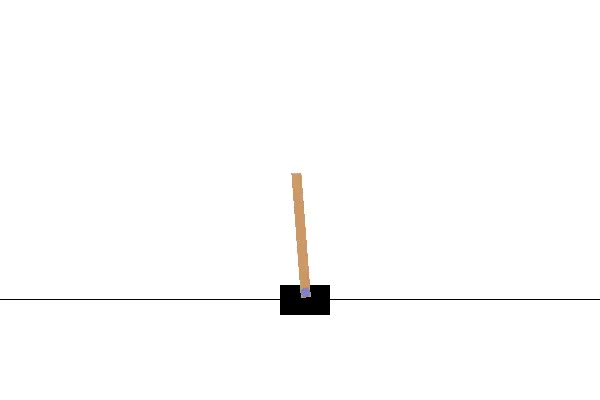
\includegraphics[width=\textwidth/2]
  {diagrams/cardpole.jpg}
  \caption{Screenshot of "CardPole-v1"}
\end{figure}

We developed our program on a HP EliteBook 8730w with a
Intel Core 2 Duo processor (2.40 GHz) running OpenSuSE
Leap 43. We needed an older Tensorflow version because the
current version does not support this CPU anymore. Also
Tensorflow was not able to utilize any GPU (Graphical
Processing Unit), which means our development environment
does not have much computing power to offer.
\index{Application!development environment}

The problem we faced with training an agent for
"CardPole-v1" was that, running the program in our
development environment, we were able to build an agent
that succeded this environment in at most three training
loops (which overall took aproximately 5 minutes). This was
achieved with running one Executor, the RabbitMQ and
between one and three Worker instances on the same device
which does not offer great computing abilitites (especially
compared to the operational environment (the cluster in
Room 1.242 containing 10 Apple Mac Pros)).
\index{Application!operational environment}

Since it would not made much sense running benchmarks on
the operational environment training an agent to master
"CardPole-v1" we needed a different Gym environment.

We decided we would take "LunarLander-v2", a Atari Arcade
Game where the agent has to land an ufo safely inside a
flagged area on the ground.
\index{OpenAI Gym!environments!LunarLander-v2}

\begin{figure}[H]
  \centering
  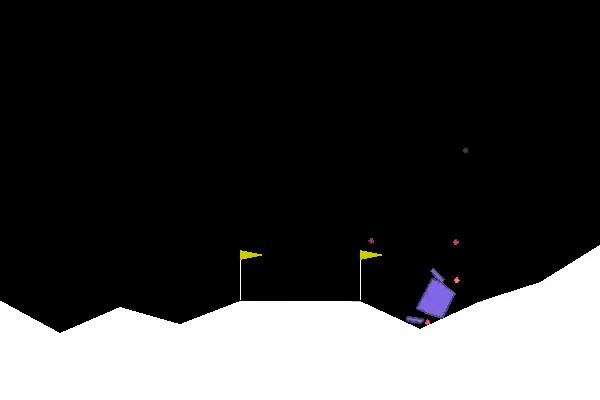
\includegraphics[width=\textwidth/2]
  {diagrams/lunarlander.jpg}
  \caption{Screenshot of "LunarLander-v2"}
\end{figure}

"LunarLander-v2" is a far more complex environment to
master since its action space is higher, it offers far more
different observations and a more complex scoring system.

When we tried to train an agent that would master
"LunarLander-v2" on our development environment we were
never able to build an agent that would succeed in this
(every time we tried running our program we canceled after
four hours of runtime).

We did four test runs on our operational environment (in
room 1.242), each with a different approach either in the
amount of Executors (one or two) or the sanitation done
to the training data (less strict which means more training
data or more strict which means higher qualitiy of the
training data).

For each test we used a neural network with two hidden
layers, both with 64 artificial neurons.

\begin{enumerate}

  \item This test run was done with a less strict policy
        toward our training data which means we took every
        episode that generated a score of over 0 and
        sanitized the episodes that had a score better than
        -400.

        Sanitation means we normalized every action's
        single score and took only the actions with a score
        better than 0.4 (we thought doing this we could
        cut out the part where the agent loses control over
        the ufo before crashing)

        We had 9 Workers running on 9 different machines
        and one Executor. Every Worker spawned 1 process
        generating training data with the agent and 5
        processes generating training data randomly.

        Every process ran 1000 Episodes.

        This test run was terminated after approximately
        one hour.

        \textbf{Observations:}

        \begin{itemize}

          \item 1000 Episodes were far too small. The
                Workers flooded the data\_queue with
                messages containing only a small amound of
                data.

          \item We discovered a very serious bottleneck.
                The messages containing the training data
                are formatted as a JSON string
                representation of a Python list which is
                parsed back into a list object when the
                Executor's main process receives it.

                But before training the list has to be
                parsed again into a format our agent (cmp.
                \ref{s_agent}) understands. The list
                containing tuples with the observation and
                the corresponding action has to be splitted
                an parsed to a NumPy Array. This parsing is
                very expensive and while doing the parsing
                the Executioner's TTSL process holds the
                shared list object (which means the main
                process has to wait until the TTSL process
                releases the list's mutex, which is one
                reason why the data\_queue was so flooded).

        \end{itemize}

  \item This time we tried to conquer the issues we faced
        in the first test run. We used the same policy
        towards our training data but increased the amount
        of episodes played by each process. Every process
        doing generation randomly now did 10000 episodes
        while the ones using the agent played 5000.

        Also now we spawned 5 processes using the agent and
        5 doing random actions.

        To avoid the bottleneck this time we added another
        Executor which roughly follows a reinforcement
        lerning technique called Double Q-Learing and is
        used to avoid overestimation for the training data
        (the agent doing the same mistakes over and over,
        because it trains with data it generated itself).
        \cite{jonas1}

        Both Executors are in a race condition for the next
        training data and both provide every Worker with
        its agent which we thought would lead to quality
        training data while keeping the data\_queue small.

        We terminated this test run after approximately
        one and three quarters of an hour, after 11
        iterations of the TTSL (both Executors). Both
        Executors combined had over 60 million data points
        and 40GB of more training data was still in the
        data\_queue.

        \textbf{Observations:}

        \begin{itemize}

          \item We only postponed the moment our
                application would kill itself with too much
                training data. Parsing again was too much.

          \item Even though we had 60 million data points
                the agents were not able to show much
                progress. Not many test runs were able to
                exceed -150 (200 being the score an episode
                is played successfully).

        \end{itemize}

  \item After having again the problem of an overflowing
        data\_queue and not much progress even after 11
        iterations we tried a stricter policy. We took only
        episodes which generated a score of over 100 and
        sanitized the episodes which had a score over -50.

        Again we used to Executors and 8 Workers, all on
        different machines.

        We terminated this test run after approximately 45
        minutes, both Executors having more than 16 million
        data points as their training data set.

        \textbf{Observations:}

        \begin{itemize}

          \item At the first iterations we had some more
                success (scores over 100 which we were
                never able to reach before), but, at the
                end, even though the Executors both had
                16 million data points, all on episodes
                with a score that had at least reached -50,
                both agents settled for test results around
                -150, like the two test runs before.

                We were not able to increase the
                performance of our agents.

        \end{itemize}

  \item We increased the strictness even more. We took only
        episodes that generated a score better than 150 and
        cut out the sanitation.

        This time we used only one Executor and again 9
        Workers.

        Again we terminated after approximately 45 minutes,
        again unsuccessful.

        \textbf{Observations:}

        \begin{itemize}

          \item Before the workers can use the agent the
                agent has to be trained with 100 percent
                random generated data. Because the policy
                was so strict the first 6 received
                messages on the data\_queue were empty. The
                seventh received message contained only 427
                data points.

          \item Like the third test run this test run had
                even greater success at the beginning,
                once actually reaching 200. But again, even
                though only training with data better than
                150 the agent settled at -150, only
                occasionally getting a better result around
                -50.

        \end{itemize}

\end{enumerate}

So, while we were able to create a distributed application
that uses a modern approach to concurrency and was able to
crunch a lot of numbers in a small amount of time,
unfortunately we were not able to build an agent that
could master "LunarLander-v2".

\subsection{Where to go, what to do next}

There are some points we would like to add to our
application in order to make it able to build an agent
that is good enough for "LunarLander-v2".

\begin{itemize}[label={}]

  \item \textbf{Statistical methods for data sanitation and
                a better agent:}

        Since we wanted to build an application that
        takes a task that takes a long time if done
        not concurrently and make it fast, we never really
        looked deeper into statistical methods from the
        fields of artificial intelligence research and
        data science that could have helped us build a
        better agent or a better training data set.

        We thought we could generate enough data to
        outweigh the weaknesses our project shows when it
        comes to optimization of agent or training data
        set.

        In the end our approach failed, so maybe by adding
        some optimizations of the agent or the training
        data set the application could be able to produce
        an agent that is able to succeed.

  \item \textbf{Some sort of load balancing:}

        We had hughe troubles in two test cases with
        an overflowing data\_queue.

        Our static approach (playing the same amount of
        episodes every iteration of the GSL (cmp.
        \ref{s_worker}) did not work that well. At some
        time the Workers start to overwhelm the
        Executor(s).

        To avoid this a unit doing load balancing should be
        added to the application that supervises the
        training data set generation using meta data from
        the Executor and the RabbitMQ.

  \item \textbf{Doing something with the parsing
                bottlneck of the Executor:}

        The parsing of the training data took longer than
        the actual training (optimized by Tensorflow).

        Right now the parsing is done in a single process
        (the TTSL process (cmp. \ref{s_executor})), however
        we think the parsing could be optimized using
        a concurrent approach (e.g. worker processes like
        we use for the data generation (cmp.
        \ref{s_worker})).

  \item \textbf{Optimize the protocolling unit:}

        The problem with our current protocolling unit is,
        that it only saves the protocol when the program
        is finished successfully, which does not help when
        failing (like we did).

        The protocolling unit should safe the data more
        often (e.g. could be integrated in the TTSL process
        (cmp. \ref{s_executor}) or a new process only for
        protocolling could be spawned).

\end{itemize}
